\graphicspath{{./Figs/}}

\chapter{Results and Discussion} 

\section{Wind Tunnel Results}

\subsection{Aerodynamic Coefficient of Lift}

\begin{figure*}
    \centering
    \begin{subfigure}[b]{0.467\textwidth}
        \centering
        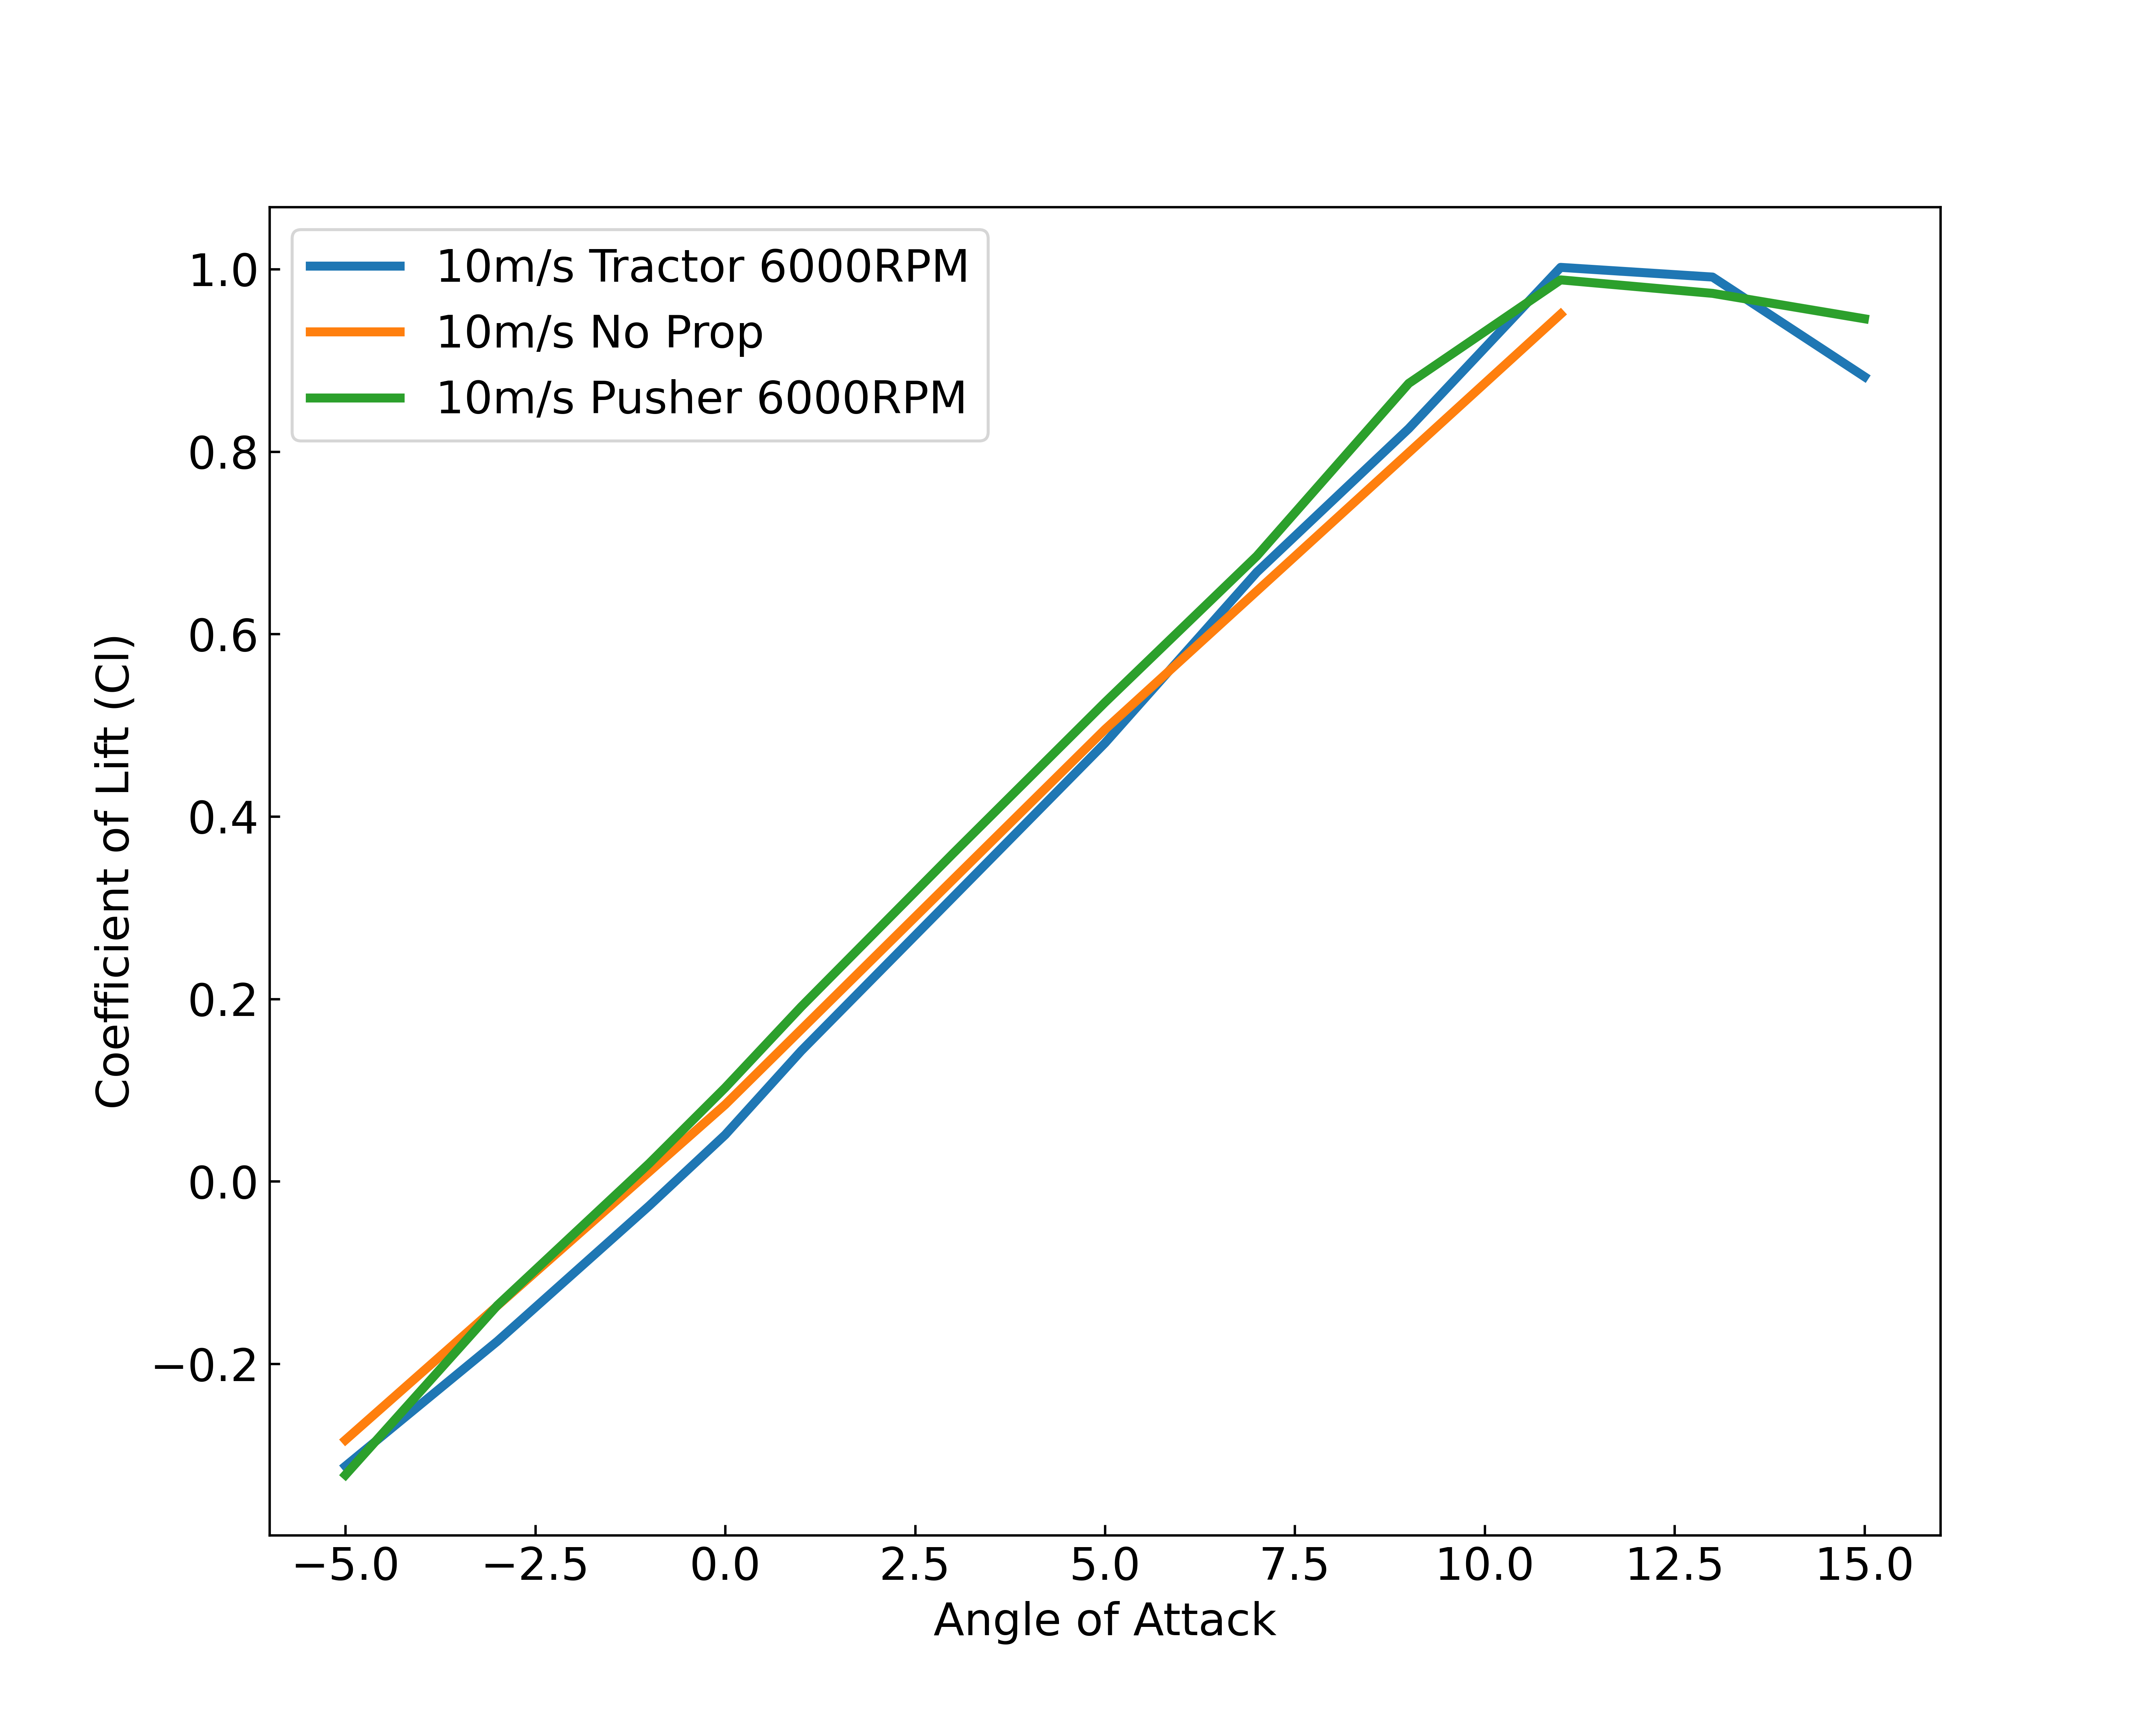
\includegraphics[width=\textwidth]{05_Results/Figs/Cl/10ms_6000RPM_Cl.png}
        \caption[Coefficient of lift at 10m/s airspeed and 6000RPM motor speed]
        \label{fig:Cl_10ms_6000}
    \end{subfigure}
    \begin{subfigure}[b]{0.467\textwidth}
        \centering
        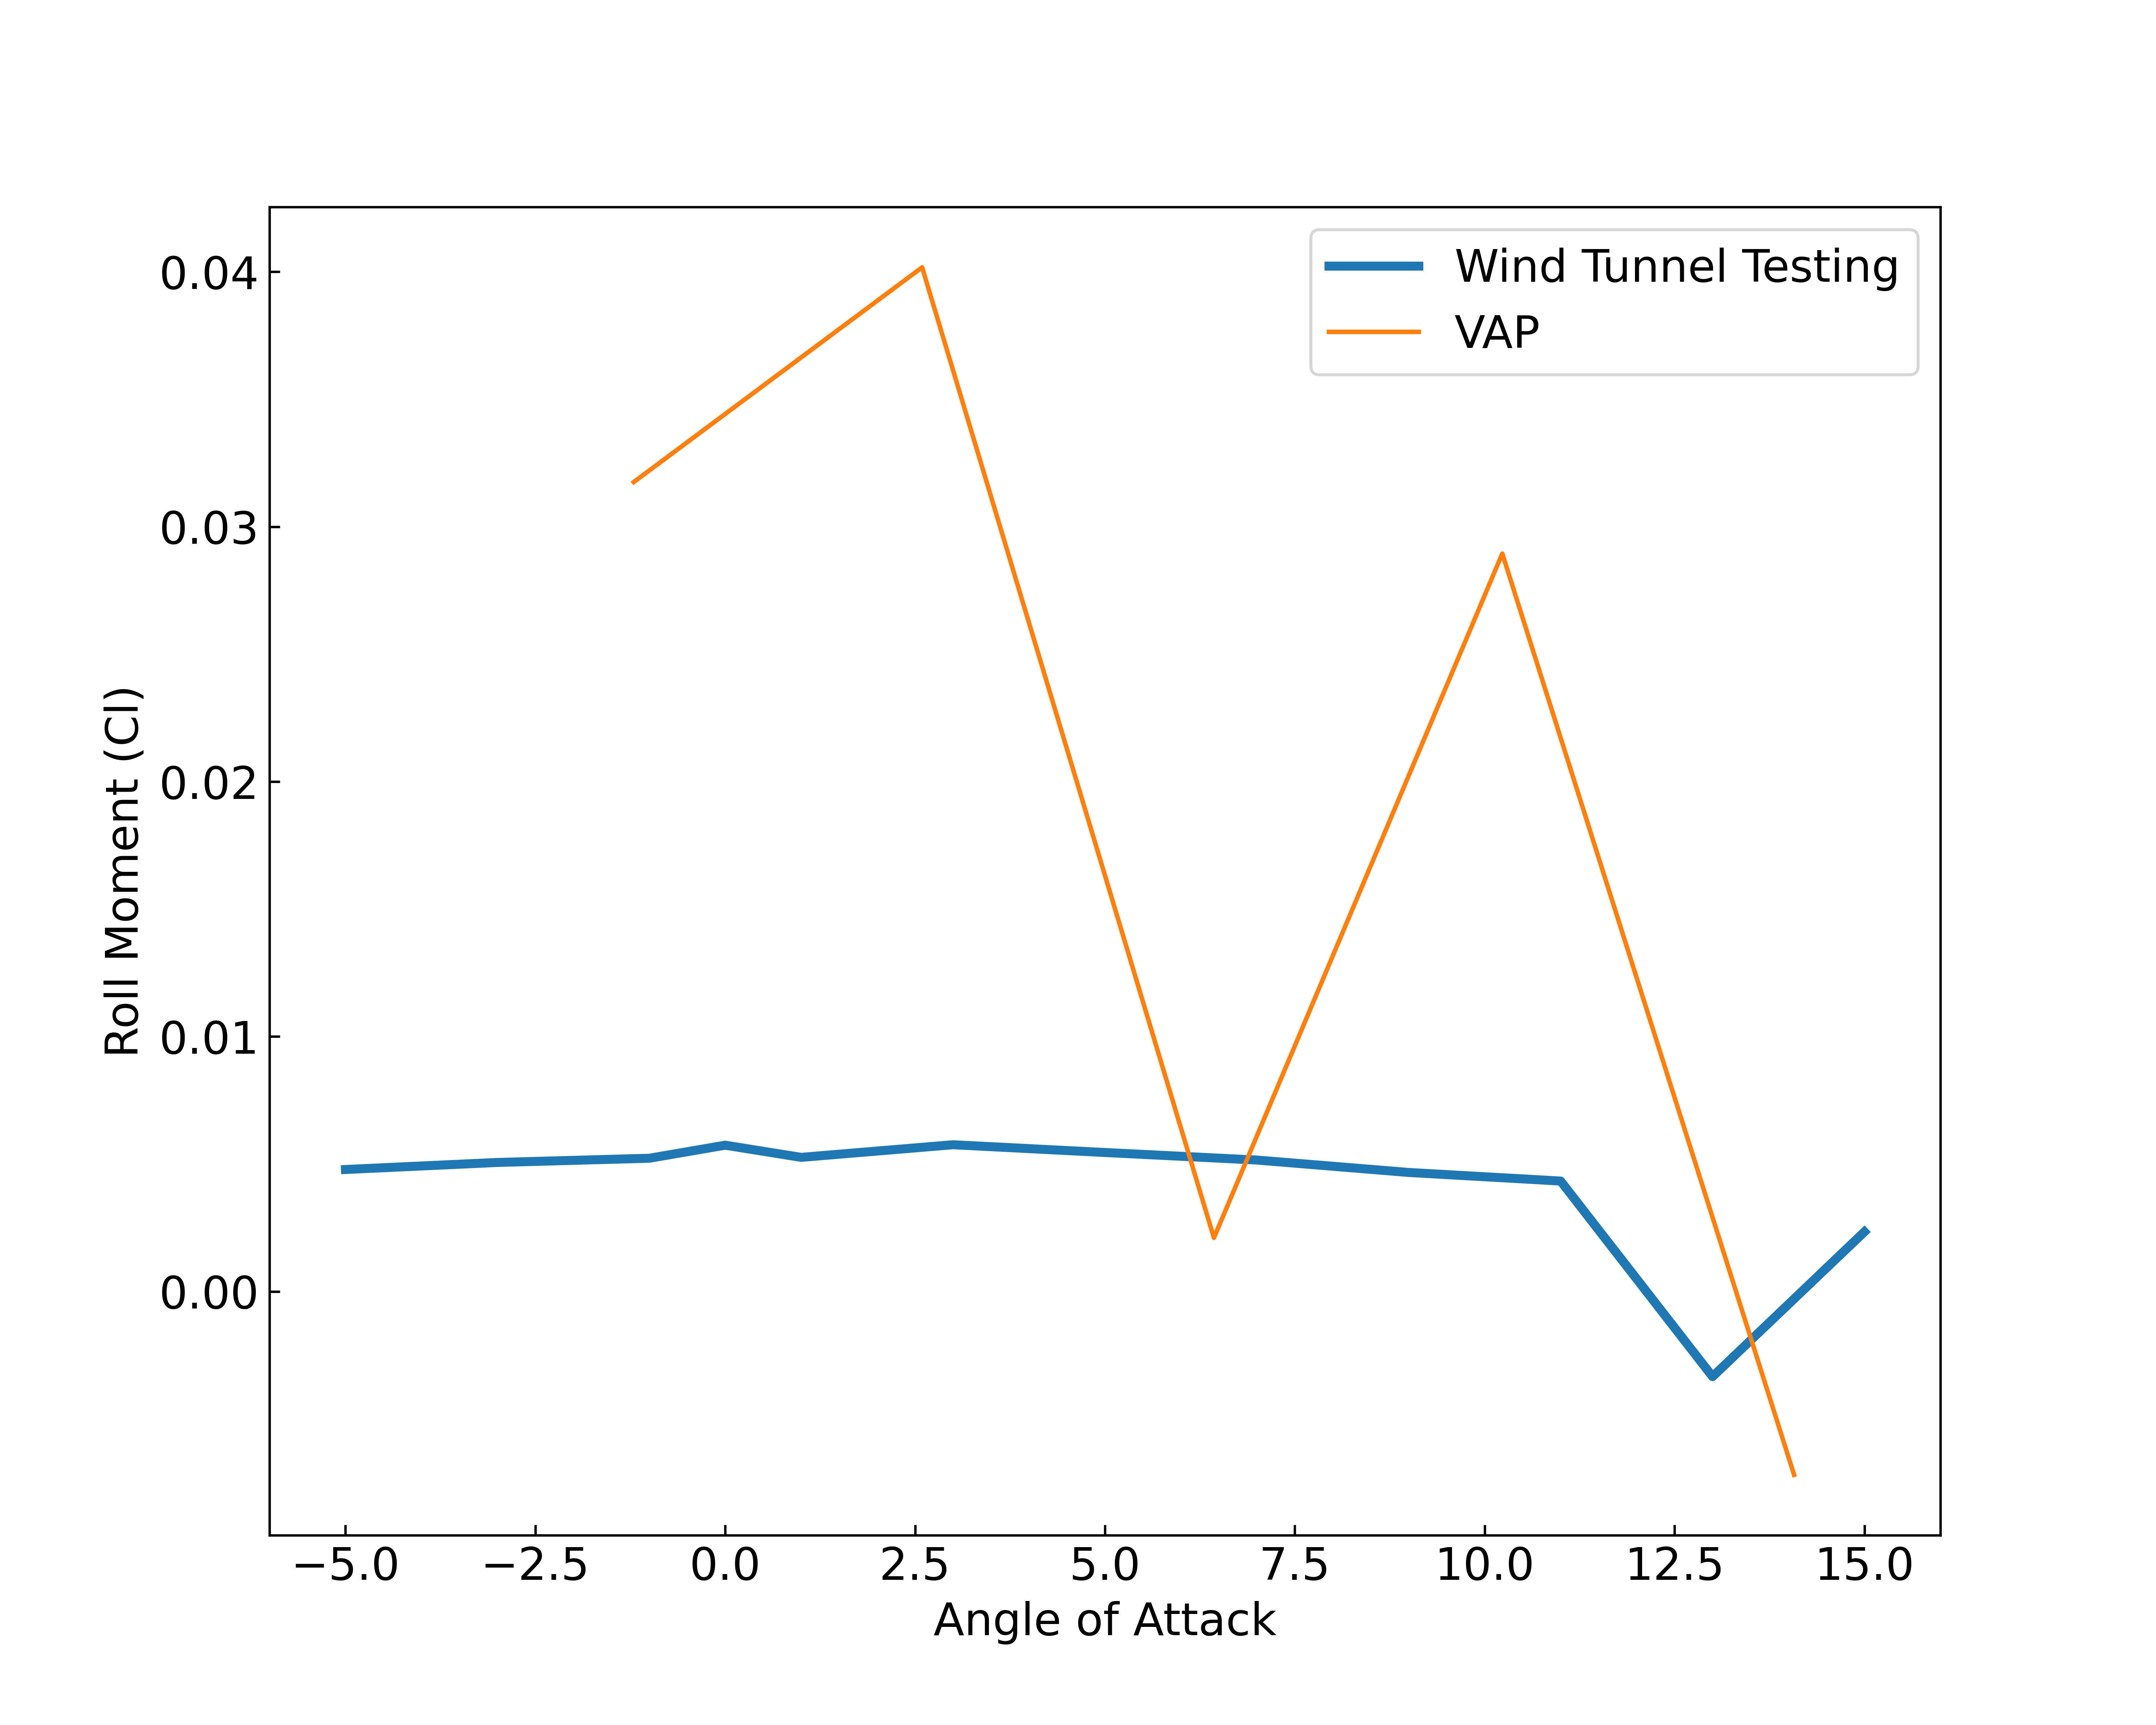
\includegraphics[width=\textwidth]{05_Results/Figs/Cl/10ms_11000RPM_Cl.png}
        \caption[Coefficient of lift at 10m/s airspeed and 11000RPM motor speed]
        \label{fig:Cl_10ms_11000}
    \end{subfigure}
    \begin{subfigure}[b]{0.467\textwidth}
        \centering
        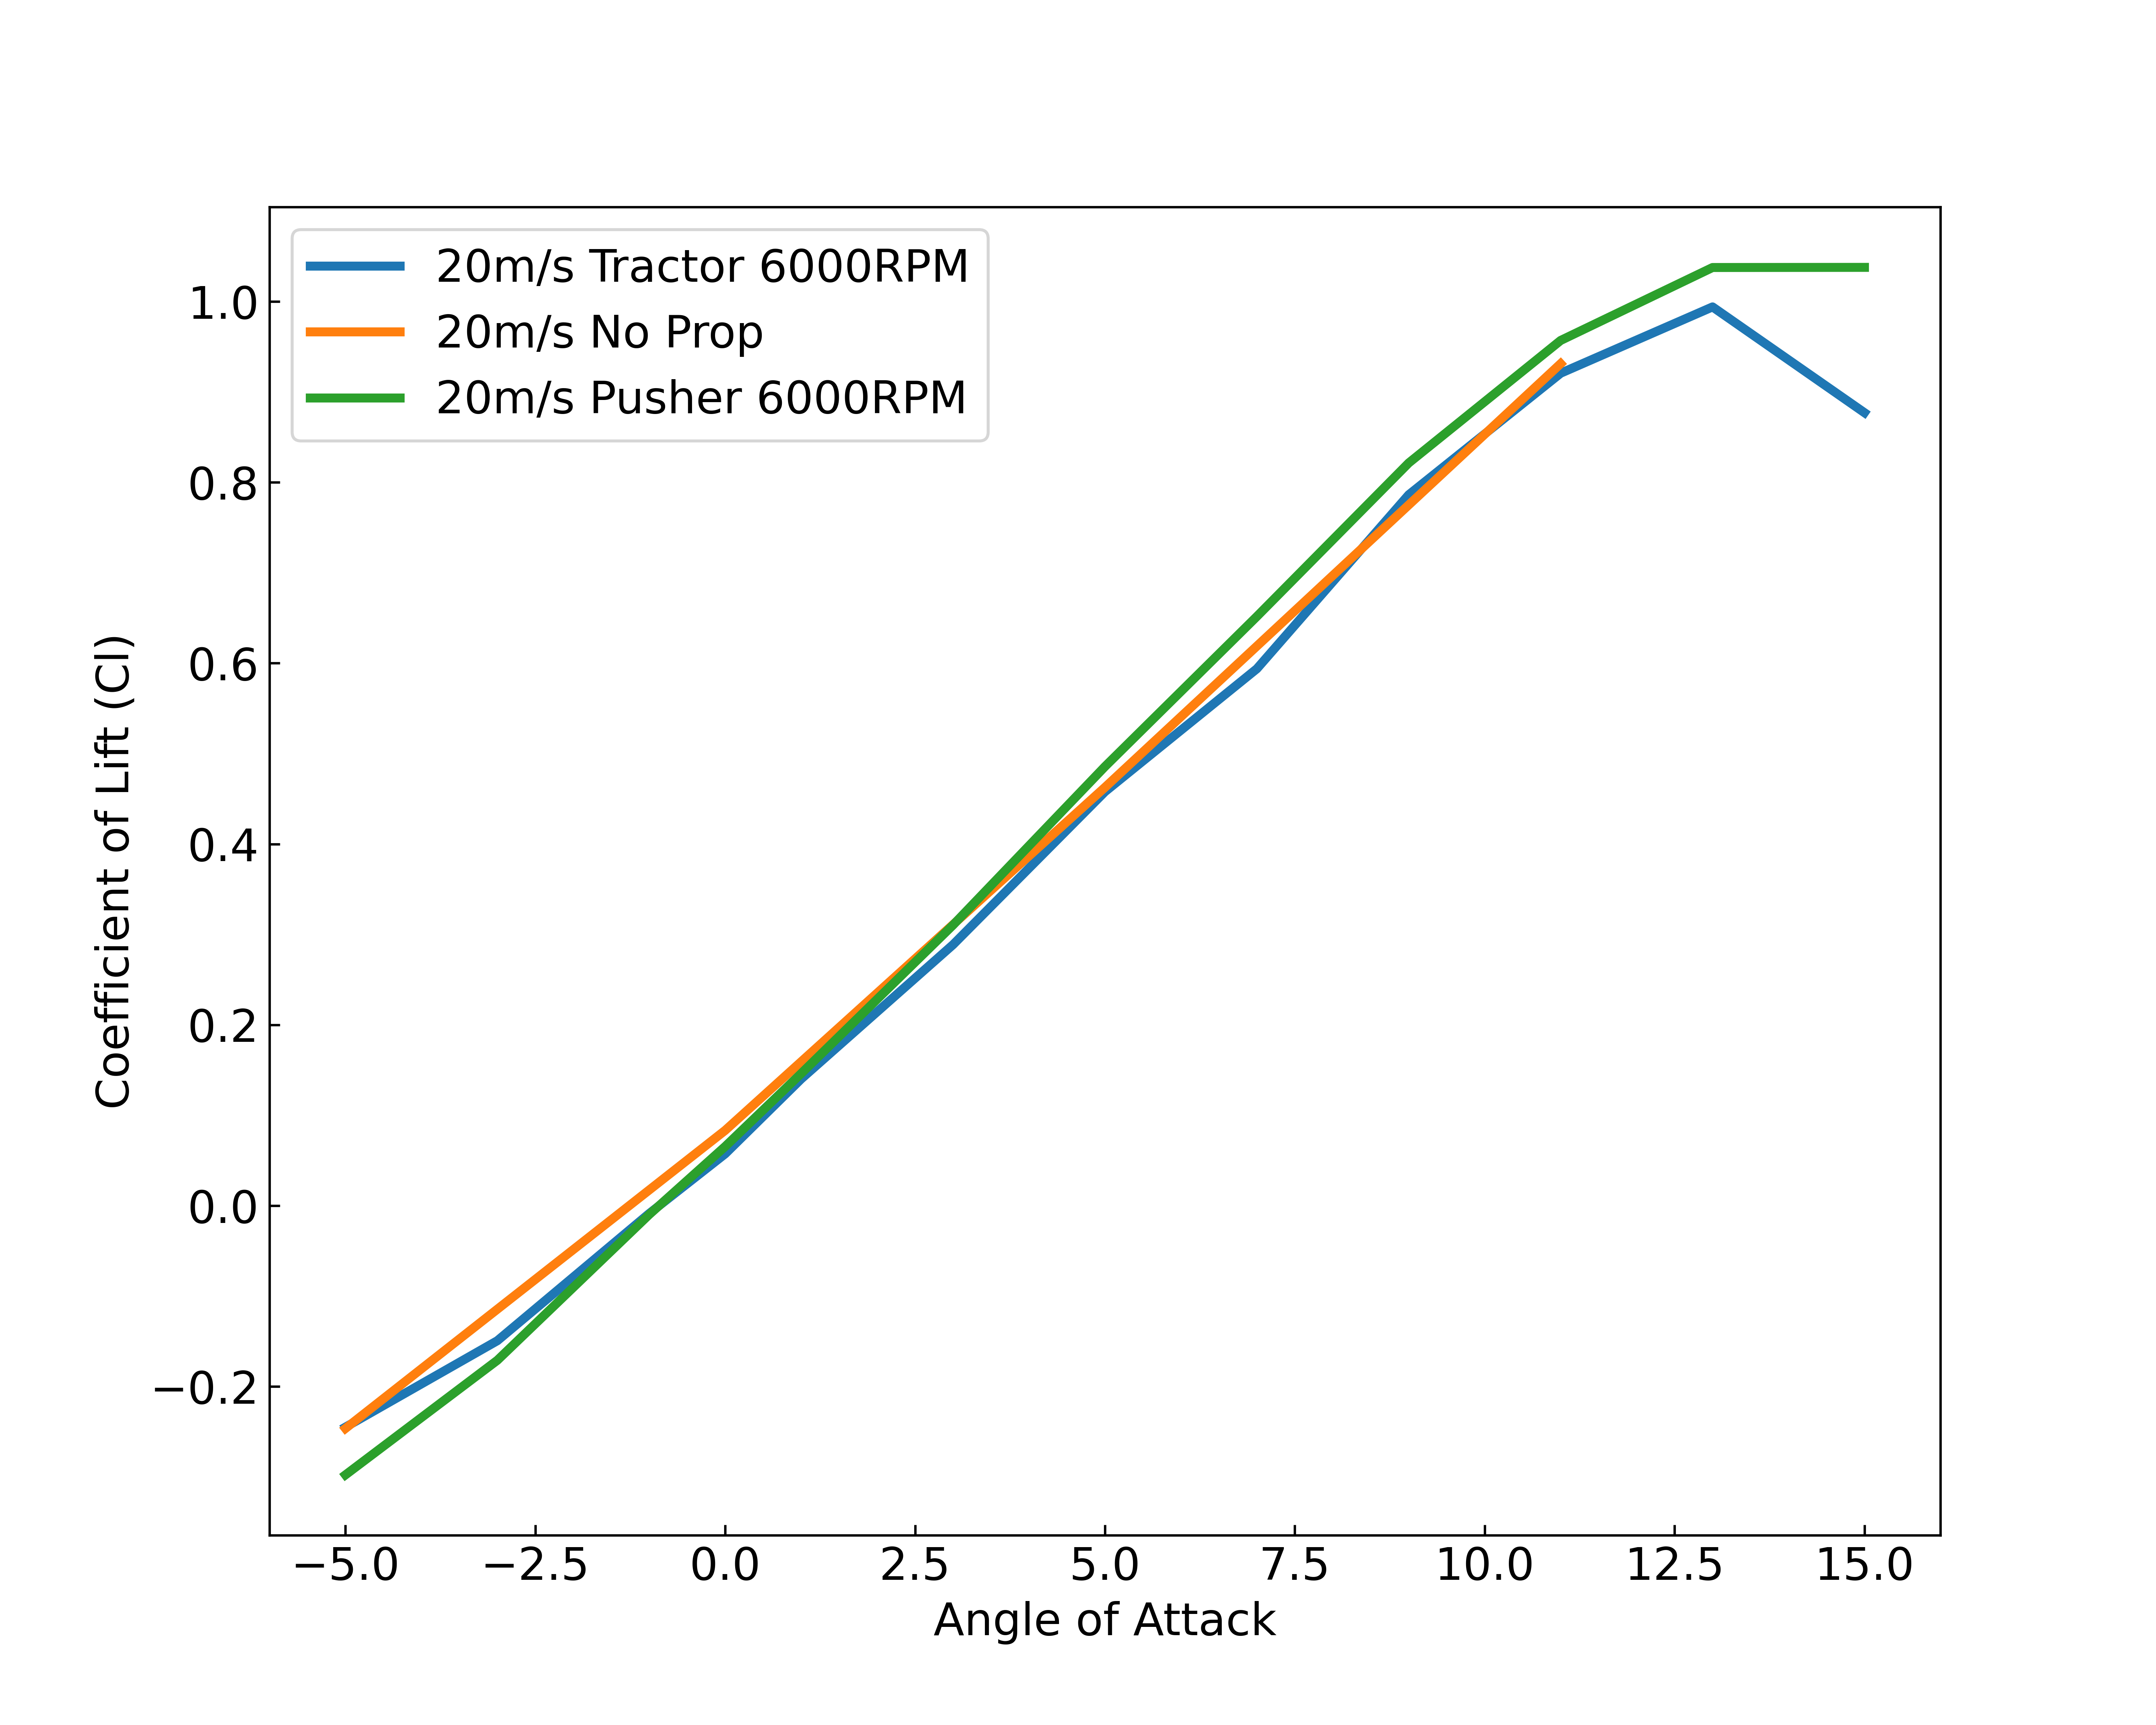
\includegraphics[width=\textwidth]{05_Results/Figs/Cl/20ms_6000RPM_Cl.png}
        \caption[Coefficient of lift at 20m/s airspeed and 6000RPM motor speed]
        \label{fig:Cl_20ms_6000}
    \end{subfigure}
    \begin{subfigure}[b]{0.467\textwidth}
        \centering
        \includegraphics[width=\textwidth]{05_Results/Figs/Cl/20ms_11000RPM.png}
        \caption[Coefficien of lift at 20m/s airspeed and 6000RPM motor speed]
        \label{fig:Cl_20ms_11000}
    \end{subfigure}
\end{figure}

\subsection{Aerodynamic Coefficient of Drag}

\subsection{Moment Coefficient o}


\section{VAP Validation}


\section{Discussion}